%______________________________________________________________________________________________________________________
% @brief    LaTeX2e Resume
\documentclass{article}
\pagestyle{empty} %no page number
\usepackage[legalpaper, top=0.5in, left=0.5in, bottom=0.4in, right=0.6in]{geometry}
\usepackage{graphicx}
\usepackage{ragged2e}
\usepackage{url}
\usepackage{hyperref}
\usepackage{marvosym}
%get rid of the ugly link color boxes
\hypersetup{
    colorlinks=false,
    hidelinks=true
}
\usepackage{amsmath}
\usepackage{amssymb}
\usepackage{titlesec}
\usepackage[scaled]{helvet}
\renewcommand\familydefault{\sfdefault} 
\usepackage[T1]{fontenc}
\usepackage{multicol}
\urlstyle{same}
\frenchspacing
\graphicspath{{./images/}}
\usepackage{enumitem}
\titleformat{\section}[block]
{\Large\bfseries}
{\thesection.}{0.5em}{}
\titlespacing{\section}{-8px}{6px}{6px}
\usepackage{xcolor}
\usepackage{colortbl}
%custom color for the horizonral rule
\definecolor{lightGray}{RGB}{191, 191, 191}
%______________________________________________________________________________________________________________________
\begin{document}
%make all bullet points small
\renewcommand{\labelitemi}{\tiny$\bullet$}
{
%Begin Header
\hspace{-12px}
\begin{minipage}[t]{0.33\textwidth}
\begin{flushleft}
\noindent
%\textbf{\huge{Devin Bonnie}}
\hspace{-15px} \textbf{\fontsize{22}{0}\selectfont Devin Bonnie}
\vspace{7px}
\linebreak
\noindent
\small{Realizing a passion for the environment by providing reliable platform capabilities through software engineering and ocean robots. Software engineer with 7+ years experience in operational robotics, software design, embedded systems, computer vision, and working closely with cross-functional teams.}
\vspace*{1\baselineskip}
\end{flushleft}
\end{minipage}
\begin{minipage}[c]{0.33\textwidth}
\begin{center}
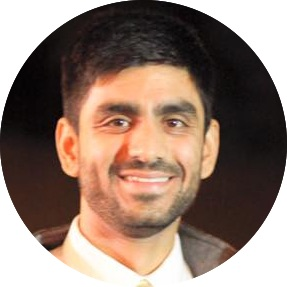
\includegraphics[trim= 0cm 8cm 0 0cm,scale=0.33]{dbCircle}
\end{center}
\end{minipage}
\begin{minipage}[t]{0.33\textwidth}
\begin{flushright}
\vspace*{1.5\baselineskip}
\href{mailto:devin.bonnie@gmail.com}{devin.bonnie@gmail.com}  \space\space \Letter
 \vspace{1px}
\linebreak
(810) 623--2687 \space\space \Telefon
 \vspace{1px}
\linebreak
Sunnyvale, CA \space\space \Mundus
 \vspace{1px}
\linebreak
\href{https://www.linkedin.com/in/devinbonnie}{linkedin.com/in/devinbonnie} \space\space 
\includegraphics[scale=0.40]{linkedin}\hspace{.9px}
\linebreak
\href{https://github.com/wriggityWrecked}{github.com/wriggityWrecked} \space\space 
\includegraphics[scale=0.225]{GitHub-Mark-32px}\hspace{1px}
\linebreak
\end{flushright}
\end{minipage}
%
\\
\textcolor{lightGray}{\rule{542px}{0.4pt}}

%End Header
\setlength{\columnsep}{32.5px}
\begin{multicols}{2}
%
%
%%__________________________________________________________________________________________________________________
    % Education
\section*{Education}
\noindent \textbf{University of Illinois at Urbana-Champaign}, Illinois\\
\textsl{M.S., Electrical and Computer Engineering}\\
\textsl{Advisor:} S.A. Hutchinson \hfill \textsl{2011}\\\vspace{0px}\\
\noindent \textbf{Hope College}, Michigan\\
\textsl{B.S., Engineering (Electrical Emphasis)}\\
Mathematics Minor \hfill \textsl{2007}\\
    \vspace{ -10px}
    \begin{itemize}[noitemsep,nolistsep]
        \item Senior project recognized with the \textit{VanPutten\\ Engineering Design Award}.
    \end{itemize}
    \vspace{5px}
    %__________________________________________________________________________________________________________________
    % Experience
\section*{Experience}
\noindent
    \textbf{Liquid Robotics, A Boeing Company}\\
    Staff Software Engineer\\
    Technical Lead \hfill \textsl{June 2017 -- Present} \\
    \vspace{ -10px}
    \begin{itemize}[noitemsep,nolistsep]
        \item Architected various components including \\naviagtional control, communications protocols, and a vehicle simulation environment.
        \item Planned releases, supervised a small team, worked directly with customers + product management, and held to deadlines.
        \item Created tools to automate system configuration and increase manufacturing throughput.
    \end{itemize}
    \vspace{10px}
    %------------------------------------------------------------------------------------------------------------
    Senior Software Engineer\\
    Technical Lead \hfill \textsl{May 2014 -- June 2017} \\
    \vspace{ -10px}
    \begin{itemize}[noitemsep,nolistsep]
    	\item Major contributor towards the entirety of the vehicle operating and control system.
         \item Operations support lead, routinely diagnosed and \\applied root cause analysis to customer-facing issues.
         \item Created live hurricane-tweeting embedded drone \\application, as a side project, that generated national news.
    \end{itemize}
    \vspace{10px}
     %------------------------------------------------------------------------------------------------------------
    Software Engineer \hfill \textsl{Aug. 2012 -- Apr. 2014}\\
    \vspace{ -10px}
    \begin{itemize}[noitemsep,nolistsep]
        \item Vehicle control system contributions included work on navigation, communications, and sensors.
        \item Integrated multiple sensors for various platforms, e.g., cameras, GPS, weather, oceanographic and \\protoyped solutions with Arduinos + Python.
        \item Contributed towards an integrator C++ API.
    \end{itemize}
    \vspace{10px}
    %------------------------------------------------------------------------------------------------------------
    \textbf{National Center for Supercomputing Applications}\\
    University of Illinois at Urbana-Champaign\\
    Research Programmer \hfill \textsl{Oct. 2011 -- Jul. 2012}\\
    \vspace{ -10px}
    \begin{itemize}[noitemsep,nolistsep]
        \item Responsibilities included computer vision image \\comparison techniques, data visualization, machine learning, and automated decision support. 
        \item Contributed to a C++ multi--conferencing and \\computer vision video library.  
        \item Other tasks included efficient incorporation/rendering of 3D image data (RGBD) over lossy network streams.  
    \end{itemize}
    \vspace{10px}
    %------------------------------------------------------------------------------------------------------------
    \textbf{University of Illinois at Urbana-Champaign}\\ 
    Dept. of Electrical and Computer Engineering\\
    Research / Teaching Assistant \hfill \textsl{Jan. 2010 -- Aug. 2011} \\
    \vspace{ -10px}
    \begin{itemize}[noitemsep,nolistsep]
	 \item Thesis work resulted in an IEEE conference \\publication titled \textsl{Probabilistic search: a Bayesian \\approach in a continuous workspace} (appeared in the May 2012 ICRA proceedings).  
        \item Assisted and lectured in senior and undergraduate courses covering robotics and circuit design. Ranked as excellent for Spring 2010, Fall 2010, and Spring 2011.
    \end{itemize}
    \vspace{10px}
    \vfill\null
    %=========
    \columnbreak
    %=========
    %------------------------------------------------------------------------------------------------------------
    \textbf{National Underwater Research Center}\\ \hfill 
	University of Connecticut\\ 
	Research Assistant \hfill \textsl{Jun. 2008 -- Feb. 2009} \\
    \vspace{ -10px}
    \begin{itemize}[noitemsep,nolistsep]
	\item Assisted with the design, implementation, and \\operation of the Kraken2 ROV.
	\item Implemented SNR reduction techniques for multiple NTSC video streams over a noisy medium.
	\item Served as main ROV engineer and pilot for NOAA's Thunder Bay Sinkhole Project. 
    \end{itemize}
    \vspace{5px}
%------------------------------------------------------------------------------------------------------------
\section*{Fellowships / Internships}
\noindent
    \textbf{Wolfram Research, Inc. }\\
     Intern \hfill \textsl{Summer 2011} \\
    \vspace{ -10px}
    \begin{itemize}[noitemsep,nolistsep]
	\item Contributed to a developmental C++ robotics API for controlling the Lego NXT. 
	\item Accomplished reliable communication, file I/O, and \\robust sensor measurement methods. 
    \end{itemize}
    \vspace{5px}
    %------------------------------------------------------------------------------------------------------------
    \textbf{Monterey Bay Aquarium Research Institute}\\
     Summer Fellow \hfill \textsl{Summer 2009}  \\
    \vspace{ -10px}	
    \begin{itemize}[noitemsep,nolistsep]
	\item Contributed to the `Software Infrastructure and \\Applications for MOOS' (SIAM) Java API by develping new instrumentation drivers and sampling protocols.
	\item Configured embedded controllers with various Linux kernels and JVMs for evaluation.
    \end{itemize}
    \vspace{5px}
    %------------------------------------------------------------------------------------------------------------
    \textbf{Great Lakes Environmental Research Laboratory}\\
    National Oceanic and Atmospheric Administration\\
    Research Assistant \hfill \textsl{Spring 2009} \\
    \vspace{ -10px}
    \begin{itemize}[noitemsep,nolistsep]
	\item Upgraded and refurbished ROV platform \\electronics for a successful ground-floor and water sampling project.
	\item Optimized underwater cabled digital video \\transmission and contributed to ReCON software \\development (C).
    \end{itemize}
    \vspace{5px}
    %------------------------------------------------------------------------------------------------------------				
    Electrical Engineer  \hfill \textsl{Summer 2007, Jan. 2008 -- Jun. 2008}  \\
    \vspace{ -10px}	
    \begin{itemize}[noitemsep,nolistsep]
	\item Collaborated with Monterey Bay Aquarium Research Institute researchers to successfully implement a testbed for emerging observing systems software.
	\item Extracted and corrected biological backscatter \\information from acoustics data to quantify \\zooplankton vertical distribution and their relation to environmental factors in the Great Lakes using Matlab and C.
    \end{itemize}
    \vspace{5px}
    %------------------------------------------------------------------------------------------------------------
    Marine Instrumentation Engineer \hfill \textsl{Summer 2006} \\
    \vspace{ -10px}	
    \begin{itemize}[noitemsep,nolistsep]
	\item Successfully automated the data retrieval process from buoy instrumentation in C. 
	\item Developed an instrument platform to support two \\analog fluorometers for \textit{in situ} sampling in C. 
    \end{itemize}
    \vspace{5px}
    %------------------------------------------------------------------------------------------------------------
    \section*{Skills} 
    \noindent
    Java, Python, C++, Google Protobufs, Git, Jira, Bash, HTML, Matlab, \LaTeXe, Maple, Mathematica, CSS, SVN, XFRACAS, Agile, Microsoft Office Suite, Adobe Photoshop, GIMP, Linux, OpenCV
    %------------------------------------------------------------------------------------------------------------
    \section*{Professional} 
    \noindent
    IEEE member of \textsl{Robotics and Automation}, \textsl{Oceanic \\Engineering}, and \textsl{Computer} Societies  
\end{multicols}
}
\end{document}
%______________________________________________________________________________________________________________________
% EOF